\documentclass[11pt,a4paper]{report}

% ---------- Packages ----------
\usepackage[utf8]{inputenc}
\usepackage[T1]{fontenc}
\usepackage{graphicx}
\usepackage[margin=1in]{geometry}
\usepackage{booktabs}
\usepackage{longtable}
\usepackage{array}
\usepackage{hyperref}
\usepackage{xcolor}
\usepackage{enumitem}
\usepackage{fancyhdr}
\usepackage{titlesec}
\usepackage{caption}
\usepackage{amsmath}
\usepackage{xurl}

\hypersetup{
    colorlinks=true,
    linkcolor=blue,
    urlcolor=blue,
    citecolor=blue,
    pdftitle={E-Commerce Visual Analytics: Technical Report},
    pdfauthor={IIT Madras -- Data Visualization Course Project Team}
}

\pagestyle{fancy}
\fancyhf{}
\fancyhead[L]{E-Commerce Visual Analytics}
\fancyhead[R]{\thepage}
\renewcommand{\headrulewidth}{0.4pt}

\titleformat{\chapter}[hang]{\normalfont\huge\bfseries}{\thechapter.}{20pt}{\Huge}

\newcommand{\finding}[1]{\par\noindent\textbf{Finding: }#1\par}
\newcommand{\takeaway}[1]{\par\noindent\textbf{Takeaway: }#1\par}
\newcommand{\caveat}[1]{\par\noindent\textit{Caveat: }#1\par}

\begin{document}

% ================= TITLE PAGE =================
\begin{titlepage}
    \centering
    \vspace*{2cm}
    {\LARGE \textbf{E-Commerce Visual Analytics}}\\[0.5cm]
    {\Large Understanding Customer Satisfaction and Retention in a Brazilian E-Commerce Marketplace}\\[2cm]

    {\large \textbf{Technical Report}}\\[0.3cm]
    {\large Data Visualization and Analytics -- Course Project}\\[0.3cm]
    {\large Indian Institute of Technology Madras}\\[2cm]

    \vfill

    {\large \textbf{Prepared by:} Project Team}\\[0.2cm]
    {\large \today}

\end{titlepage}

\tableofcontents
\listoffigures
\clearpage

% ================= ABSTRACT =================
\chapter*{Abstract}
\addcontentsline{toc}{chapter}{Abstract}

This report presents an end-to-end visual-analytics study of a Brazilian e-commerce marketplace
dataset (Olist-style order, customer, seller, product-category, and review data) combined with a
marketing-funnel dataset describing how sellers are acquired. The project's central business
question is: \textit{why does only about 3.1\% of the customer base ever return for a second
order, and where should the marketplace intervene to fix it?}

The analysis proceeds from raw-data cleaning and table construction, through exploratory analysis
at the order, customer, seller, and category levels, to an explanatory narrative that traces
dissatisfaction from customer reviews down to specific states, sellers, and product categories,
and finally back up to a sized, revenue-weighted customer segment. Across every level of
granularity examined, \textbf{delivery delay is the most consistent and strongest correlate of
customer dissatisfaction} -- late orders average a review score of 2.27--2.3 versus 4.16--4.29 for
on-time orders, and this pattern holds at the order, customer, and seller level alike. A small,
identifiable set of sellers, product categories (bulky/fragile goods), and states (Alagoas, Rio de
Janeiro) account for a disproportionate share of the problem. A revenue-weighted customer segment
of roughly 4{,}200 ``high-value and unhappy'' customers (11.3\% of total revenue) is identified as
the single highest-leverage group for intervention, since their late-delivery rate
(\textasciitilde26\%) is roughly 8x that of comparably valuable, satisfied customers
(\textasciitilde3\%).

All findings are explicitly framed as \textit{associations}, not proven causal effects, in line
with the limits of observational marketplace data; recommendations are presented as the
best-supported next actions to test operationally, not settled facts.

\clearpage

% ================================================================
\chapter{Introduction}
% ================================================================

\section{Business Context}
The marketplace under study connects a large base of small and medium sellers with retail
customers across Brazil. Between 2016-09-15 and 2018-08-29, the platform processed \textbf{95{,}830
orders} from \textbf{96{,}096 unique customers}, fulfilled by \textbf{3{,}095 active sellers},
generating a Gross Merchandise Value (GMV) of \textbf{R\$13{,}109{,}390.63} and collecting
\textbf{R\$2{,}181{,}332.34} in freight, for an average order value of \textbf{R\$159.59}.

At a glance, the marketplace looks healthy: 99.99\% of orders were successfully delivered
(0.01\% cancelled), the marketplace-wide average review score is \textbf{4.16 / 5}, and the
marketplace-wide late-delivery rate is a modest \textbf{6.66\%}. However, a closer look at customer
behavior reveals a much more urgent problem.

\section{The Core Business Question}
Only \textbf{3.1\% of customers} placed more than one order in the observed period; \textbf{96.9\%}
made a single purchase and never returned. This project was scoped around a single driving
question:

\begin{quote}
\textit{Why do so few customers come back, and which specific, actionable levers -- delivery,
sellers, product categories, or acquisition channels -- would move that number?}
\end{quote}

\section{Scope and Datasets}
The analysis draws on six cleaned, analysis-ready tables, each built from raw Olist-style
e-commerce data plus a separate marketing-funnel dataset:

\begin{itemize}[leftmargin=2em]
    \item \textbf{Master order table} (95{,}830 rows) -- one row per order, covering timestamps,
        delivery performance, freight, and review fields.
    \item \textbf{Customer-level master table} (96{,}096 rows) -- one row per customer, aggregating
        lifetime order count, spend, delivery experience, and review behavior.
    \item \textbf{Seller-level master table} (3{,}095 rows) -- one row per seller, aggregating
        sales volume, delivery reliability, and review risk.
    \item \textbf{Category-level master table} (73 rows) -- one row per product category, rolling
        up sales volume and satisfaction/delivery metrics.
    \item \textbf{Marketing-funnel table} (8{,}000 rows) -- one row per marketing-qualified lead,
        tracking acquisition channel and conversion to seller.
    \item \textbf{Processed customer reviews} -- sentiment- and topic-mined free-text reviews,
        translated from Portuguese to English, used to explain \textit{why} customers were
        dissatisfied.
\end{itemize}

The full data-preparation and per-table exploratory work is summarized in Chapters 2 and 3; the
explanatory narrative that answers the core business question is presented in Chapter 4.

\clearpage

% ================================================================
\chapter{Data Preparation}
% ================================================================

This chapter summarizes the cleaning and feature-engineering decisions behind each of the six
tables used in the analysis. Full detail and code are in the corresponding cleaning notebooks
(see Appendix~A for links).

\section{Master Order Table}
\textbf{Cleaning notebook:} \path{data_cleaning/cleaning_master_order_table.ipynb}

Raw order, customer, and review data were joined into a single order-level table. Two small
null-handling decisions were made explicitly rather than silently:
\begin{itemize}
    \item \path{order_approved_at} (14 nulls) and \path{order_delivered_carrier_date}
        (1 null) were imputed using the median approval delay, since the gap between adjacent
        timestamp columns is small and stable enough for a median-based fill to be defensible.
    \item Rows with no \path{review_score} were dropped rather than imputed, since a review
        score cannot be meaningfully guessed from other columns without fabricating signal.
    \item Orders that never reached the customer (no \path{order_delivered_customer_date})
        had \path{actual_delivery_days} and \path{delivery_delay_days} left null and
        excluded from delivery-timing statistics, rather than being backfilled with a guessed
        delivery date.
\end{itemize}

Engineered columns include \path{approval_delay_days}, \path{shipping_prep_days},
\path{transit_days}, \path{total_delivery_days}, \path{delivery_vs_estimate_days},
\path{late_delivery_flag}, and calendar features (\path{purchase_year},
\path{purchase_month}, \path{purchase_dow}, \path{purchase_hour}). Outliers in numeric
columns were identified via the IQR method and capped (not dropped) into separate
\path{_capped} columns, preserving the original values so that outlier sensitivity could be
checked rather than assumed away. The cleaned table was ultimately split into two
sub-tables -- \path{cleaned_master_order_table1.csv} (customer/order/review identity fields)
and \path{cleaned_master_order_table2.csv} (order-economics fields: freight, item count,
seller count) -- to keep each table focused.

\section{Customer-Level Master Table}
\textbf{Notebook:} \path{data-visualization/customer-master-analysis.ipynb}

Built by aggregating the order table to one row per \path{customer_unique_id}: total orders,
total/average payment value, average review score, late-delivery rate, product/seller diversity,
and a \path{repeat_customer_flag}. A known limitation, explicitly documented rather than
hidden, is that this table aggregates each customer's \emph{entire observed history} into one row,
so the \textasciitilde3.1\% repeat rate should be read as a lower bound partly shaped by the
observation window (customers who joined near the end of the window have had less time to
re-order), not purely by product or service quality.

\section{Seller-Level Master Table}
\textbf{Cleaning notebook:} \path{data_cleaning/clean_seller_master_table.ipynb}

One row per seller (3{,}095 rows, 28 raw columns), aggregating order volume, sales value, delivery
performance, and review behavior. The key missing-value decision: \path{avg_review_score} is
missing exactly when \path{review_count} is 0 (a seller with no reviews yet). Rather than
imputing a fabricated score, the row is kept and a \path{has_reviews} flag is added, so
downstream analyses can exclude unreviewed sellers cleanly instead of treating a missing score as
a zero. A data-quality issue was also identified and flagged rather than silently used:
\path{active_seller_flag} is \path{True} for 100\% of rows and currently carries no
discriminating information -- it should not be used for any ``active vs.\ inactive'' filtering
until fixed upstream.

\section{Category-Level Master Table}
\textbf{Cleaning notebook:} \path{data_cleaning/clean_category_master_table.ipynb}

Built by joining order items to products and translating category names to English, then rolling
up to 73 categories with sales volume, seller count, and the same satisfaction/delivery metrics
used elsewhere. Only 610 products (1.9\% of the raw catalog) with no category at all were dropped;
the 73 surviving categories have complete, non-imputed \path{has_reviews} and
\path{has_delivery_data} coverage. Two categories (\path{pc_gamer},
\path{portateis_cozinha_e_preparadores_de_alimentos}) have no official English translation
and are kept under their Portuguese name -- a labeling quirk only, not a data-quality gap.

\section{Marketing-Funnel Table}
\textbf{Cleaning notebook:} \path{data_cleaning/clean_marketing_funnel_table.ipynb}

One row per marketing-qualified lead (8{,}000 leads), with \path{is_converted_flag} set when a
matching closed deal exists. Two cleaning decisions stand out:
\begin{itemize}
    \item \path{declared_monthly_revenue} and \path{declared_product_catalog_size} were
        found to be exactly 0 for \textasciitilde95\% of converted deals -- a pattern uniform
        across every lead type, consistent with an unanswered survey field defaulting to 0 rather
        than a real declared value. These were recoded to \path{NaN} with explicit
        \path{has_declared_revenue} / \path{has_declared_catalog_size} flags, leaving only
        45 of 842 converted deals (5.3\%) with a usable, non-placeholder revenue figure.
    \item One converted deal showed a negative \path{time_to_win_days} (recorded as won two
        days \emph{before} first contact) -- almost certainly an upstream data-entry error. It was
        flagged via \path{time_to_win_valid_flag} and excluded from timing statistics rather
        than silently kept or dropped from the table entirely.
    \item Deal-side fields (\path{business_segment}, \path{lead_type},
        \path{business_type}, \path{sdr_id}, \path{sr_id}, \path{won_date}) are
        \path{NaN} precisely when \path{is_converted_flag} is \path{False}, by construction
        of the join -- a missing value there means ``never converted,'' not ``dirty data.''
\end{itemize}

\section{Customer Reviews (Sentiment and Topic Mining)}
\textbf{Notebook:} \path{EDA/review_message_analysis.ipynb}

Review titles and messages, originally in Portuguese, were translated to English, combined into a
single text field, and passed through sentiment classification and topic classification to
identify recurring complaint themes (delivery delay, product condition/damage, product quality,
returns/refunds, etc.). This structured output (\path{sentiment}, \path{primary_topic}) is the
join key used throughout Chapter 4 to connect qualitative complaints to quantitative delivery and
seller/category metrics.

\clearpage

% ================================================================
\chapter{Exploratory Data Analysis}
% ================================================================

This chapter summarizes the exploratory findings from each table, prior to being woven into the
explanatory narrative in Chapter 4. Full question-by-question detail with all supporting numbers
is preserved in the per-table Q\&A documents (Appendix~A).

\section{Order-Level Findings}
\begin{itemize}
    \item Total delivery time is heavily right-skewed: most deliveries complete in 5--15 days,
        with a long tail out to 40--50 days.
    \item \textbf{Delivery delay is the strongest driver of review score at the order level.}
        On-time orders average \textbf{4.29}; late orders average \textbf{2.27}, and \textbf{53.78\%}
        of late orders receive a 1-star review (vs.\ 6.62\% for on-time orders). Banding by exact
        delay shows a consistent dose-response pattern: 1--2 days late $\rightarrow$ 3.51,
        3--5 days $\rightarrow$ 2.47, 6--10 days $\rightarrow$ 1.77, $>$10 days $\rightarrow$ 1.71.
    \item Order complexity matters independently of lateness: 1-item orders average 4.21 (8.50\%
        1-star) vs.\ 3.25 (31.69\% 1-star) for 6+-item orders, despite late-delivery rates staying
        flat across this range -- larger, more complex orders are simply less satisfying, not just
        more delay-prone.
    \item Multi-seller orders score worse (2.89 for 2 sellers, 2.24 for 3+) \emph{despite} lower
        observed late-delivery rates -- suggesting the coordination overhead of split shipments is
        a distinct dissatisfaction driver, not one mediated by lateness.
    \item SP (S\~ao Paulo) accounts for roughly 3.5x the order volume of the next-largest state.
\end{itemize}

\section{Customer-Level Findings}
\begin{itemize}
    \item Customer revenue is spread across volume, not concentrated among ``whale'' customers:
        the top 20\% of customers generate \textasciitilde54\% of revenue, and the median customer
        spends only R\$108.
    \item Delivery experience is the single strongest signal in the customer-level data: customers
        whose orders are mostly late average \textasciitilde2.3 on review score vs.\
        \textasciitilde4.2 for mostly-on-time customers, beating every other tested candidate
        variable (payment behavior, basket diversity).
    \item Raw delivery \emph{speed} matters even after controlling for lateness: even restricting
        to on-time deliveries only, orders under 7 days score 4.42 vs.\ 3.86 for orders over 21
        days -- ``don't be late'' is necessary but not sufficient; genuinely fast delivery earns an
        additional satisfaction premium.
    \item Payment installments and basket/seller diversity are only weak, secondary signals
        (seller-diversity vs.\ late-rate correlation \textasciitilde$-0.01$) -- delivery reliability
        dominates the picture so thoroughly that these barely register by comparison.
\end{itemize}

\section{Seller-Level Findings}
\begin{itemize}
    \item Sellers are heavily concentrated in S\~ao Paulo (1{,}849 of 3{,}095, 60\%).
    \item Sales are long-tail: the top 10\% of sellers generate 67.5\% of item sales value.
    \item Late-delivery rate correlates with average review score at $-0.42$ across sellers, and
        with the derived \path{review_risk_rate} at $+0.40$.
    \item Most sellers (97\%) beat their own delivery estimate on average, but a real tail exists:
        230 sellers (7.4\%) have a late-delivery rate above 20\%.
    \item Seller tenure has essentially no relationship with review score ($+0.08$) or late-delivery
        rate ($+0.01$) -- longevity on the platform does not by itself predict quality.
    \item Sellers in outlying states (PE, CE, PB, MA, MT) pay a structurally higher freight-to-sales
        ratio (32--36\%) than the national average (26.5\%), a geography-driven cost that should be
        controlled for when comparing seller efficiency across regions.
\end{itemize}

\section{Category-Level Findings}
\begin{itemize}
    \item Category revenue is long-tail: the top 10 of 73 categories generate \textasciitilde63.2\%
        of total sales value.
    \item Category size and category satisfaction are essentially uncorrelated ($\sim$0.01) -- a
        large category is not automatically ``safe,'' and a small one is not automatically
        low-risk.
    \item \path{office_furniture} stands out as the most important category to act on: it does
        real volume (1{,}654 reviews, R\$273{,}961 in sales) yet scores meaningfully below the
        marketplace average (3.51 vs.\ \textasciitilde4.08).
    \item At the category-aggregate level, the delivery--satisfaction link is much weaker
        ($\sim -0.05$) than at the order or seller level -- consistent with other factors (product
        type, price point, seller mix within category) diluting the signal when averaged across an
        entire category; delivery is still the right lever, but should be diagnosed within a
        category, not from the category-level correlation alone.
\end{itemize}

\section{Marketing-Funnel Findings}
\begin{itemize}
    \item Overall lead-to-seller conversion is \textasciitilde10.5\% (842 of 8{,}000 leads); this is
        not a ``still warming up'' artifact, since converted and unconverted leads have
        near-identical age distributions.
    \item Channel volume and channel quality diverge: \path{organic_search} and
        \path{paid_search} bring the most leads, but \path{unknown} (untracked referral) and
        \path{paid_search} convert best; \path{social} and \path{email} carry real volume
        (300+ leads each) but convert well below average.
    \item Converted leads skew \textasciitilde2:1 toward \path{reseller} over
        \path{manufacturer} business type, confirming the marketplace's structural role as a
        platform for small/medium resellers.
    \item Median time-to-win is about two weeks, with a long right tail past 100+ days for a small
        group of ``stuck'' leads.
\end{itemize}

\clearpage

% ================================================================
\chapter{Explanatory Analysis: The Retention Story}
% ================================================================

This chapter presents the project's central narrative, built in \path{combined_eda.ipynb}: a
single, connected walk from the retention problem, through customer complaints, to specific
geographic, seller, and category-level causes, back up to a sized customer segment and a set of
recommendations. Figures are numbered in narrative order; each live (re-executed) chart is
paired with the specific numbers it supports.

\section{The Retention Problem}

Of 96{,}096 customers, only \textbf{3.1\%} placed more than one order; \textbf{96.9\%} made a
single purchase and never returned (Figure~\ref{fig:repeat_pie}).

\begin{figure}[htbp]
    \centering
    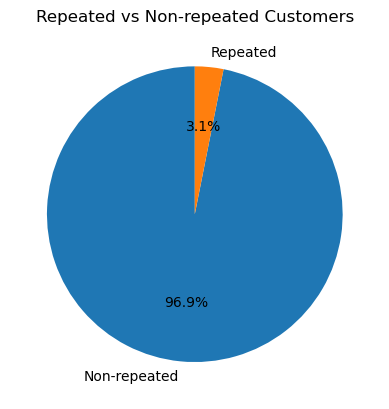
\includegraphics[width=0.55\textwidth]{figures/f_repeat_customer_pie.png}
    \caption{Repeated vs.\ non-repeated customers (3.1\% vs.\ 96.9\%).}
    \label{fig:repeat_pie}
\end{figure}

\takeaway{The platform is effective at acquiring customers but has an almost entirely untapped
retention problem. This raises the driving question: why are so many customers not returning?}

\section{What Are Dissatisfied Customers Complaining About?}

Restricting to one-time customers and their \emph{negative}-sentiment reviews, the dominant
complaint themes are \textbf{delivery delay} (915 reviews), \textbf{product condition/damage}
(808), \textbf{product quality} (397), and \textbf{return/refund} issues (365), alongside a large
``Other'' bucket (1{,}841) (Figure~\ref{fig:neg_topics}).

\begin{figure}[htbp]
    \centering
    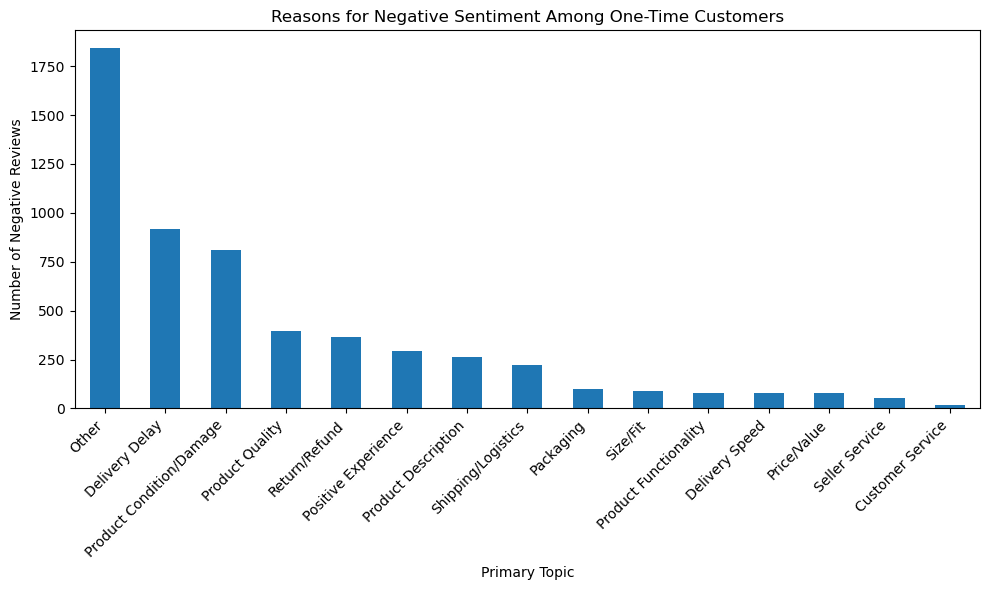
\includegraphics[width=0.85\textwidth]{figures/f_negative_review_topics.png}
    \caption{Reasons for negative sentiment among one-time customers, by primary review topic.}
    \label{fig:neg_topics}
\end{figure}

\finding{Delivery reliability and product-related issues are the two largest, most actionable
complaint categories.}
\caveat{The presence of these complaints does not by itself establish that they \emph{caused}
customers not to return. The remainder of this chapter tests whether these themes are actually
associated with satisfaction, delivery performance, and repeat behavior.}

\section{Geographic Analysis: Delivery Reliability vs.\ Scale}

\begin{figure}[htbp]
    \centering
    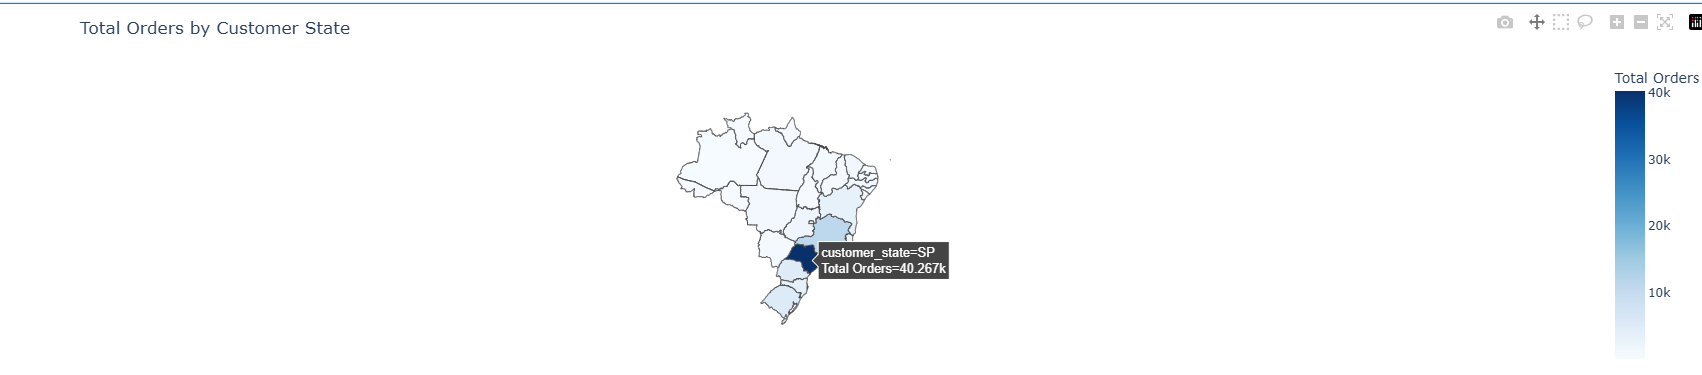
\includegraphics[width=0.85\textwidth]{figures/f_orders_by_state_choropleth.png}
    \caption{Total orders by customer state (choropleth).}
    \label{fig:orders_choropleth}
\end{figure}

\begin{figure}[htbp]
    \centering
    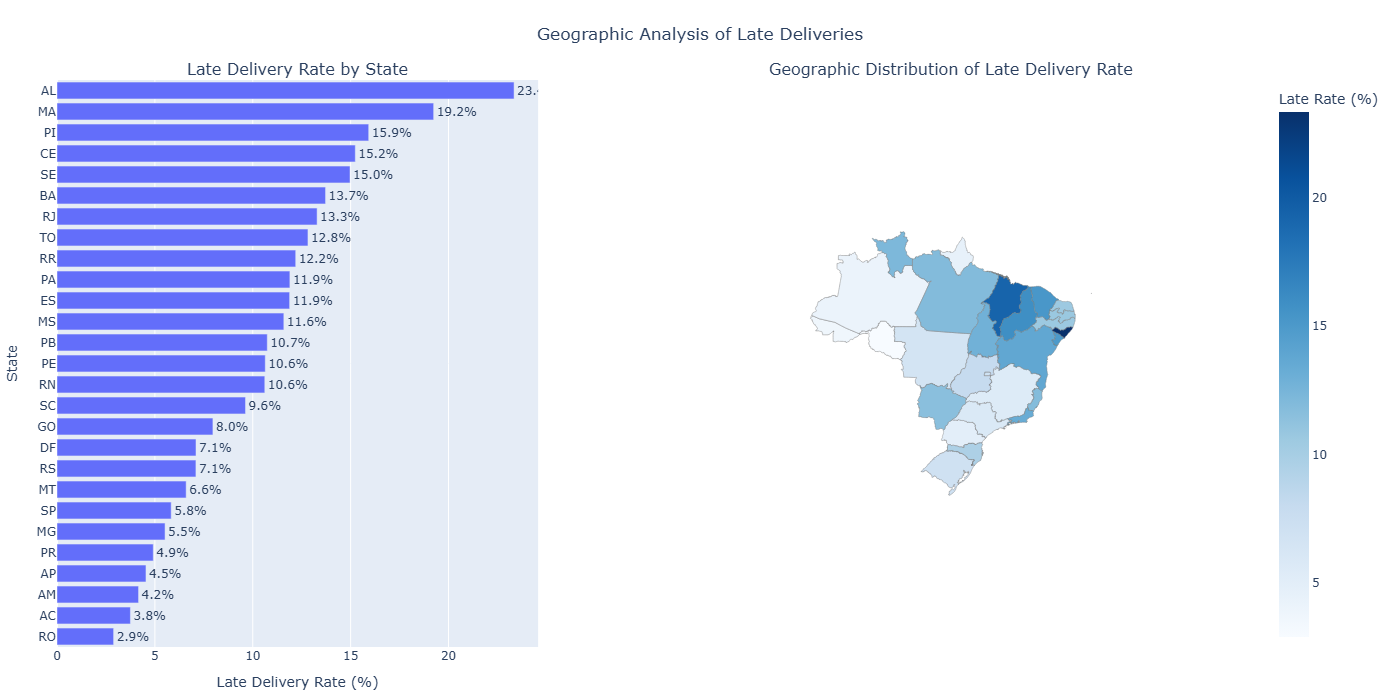
\includegraphics[width=0.85\textwidth]{figures/f_late_rate_by_state_original.png}
    \caption{Late-delivery rate by state -- bar chart and choropleth (original analysis).}
    \label{fig:late_rate_orig}
\end{figure}

\begin{figure}[htbp]
    \centering
    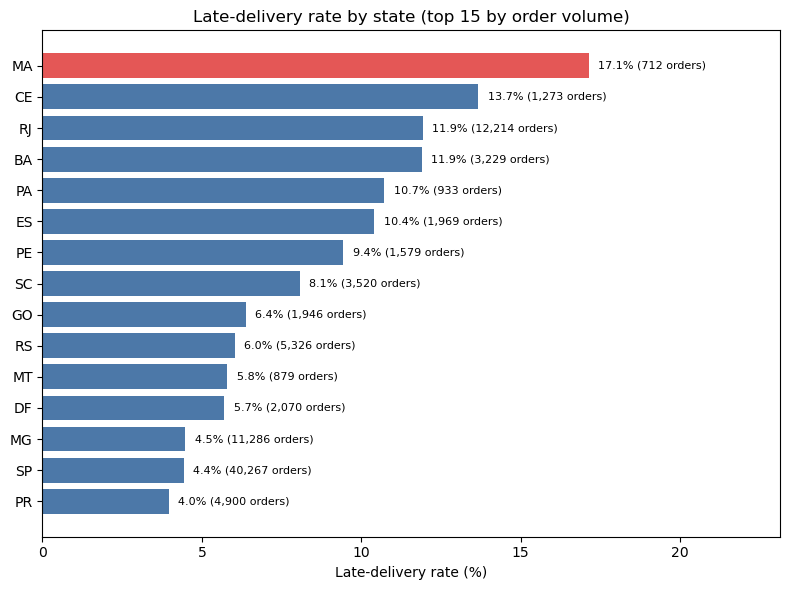
\includegraphics[width=0.75\textwidth]{figures/f_late_rate_by_state_recompute.png}
    \caption{Late-delivery rate by state, top 15 states by order volume (live recomputation).
    States highlighted in red (AL, MA, PI) are the low-seller-density, high-late-rate states
    discussed in Section~4.4.}
    \label{fig:late_rate_recompute}
\end{figure}

Live recomputation confirms and sharpens the original finding: \textbf{Alagoas (AL)} has the
worst late-delivery rate at \textbf{20.8\%} (394 orders), followed by \textbf{Maranh\~ao (MA)}
at \textbf{17.1\%} and \textbf{Sergipe (SE)} at \textbf{15.0\%}. Among high-volume states,
\textbf{Rio de Janeiro (RJ) stands out at 11.9\%} -- nearly 3x S\~ao Paulo's rate despite RJ being
the \emph{second-largest} market by order count (12{,}214 orders). S\~ao Paulo (SP) itself sits at a
low \textbf{4.4\%} despite handling by far the most orders (40{,}267).

\finding{The marketplace faces two distinct delivery problems, not one: AL/MA/SE/PI have a
\emph{reliability} problem despite low volume, while RJ has a \emph{reliability} problem
\emph{despite} high volume and (as shown next) a reasonably deep seller base -- a hidden problem
inside a big market that the ``small state = logistics problem'' framing would miss. SP, in
contrast, demonstrates that high volume does not have to mean poor reliability.}

\section{Seller Supply and Geographic Reliability}

\begin{figure}[htbp]
    \centering
    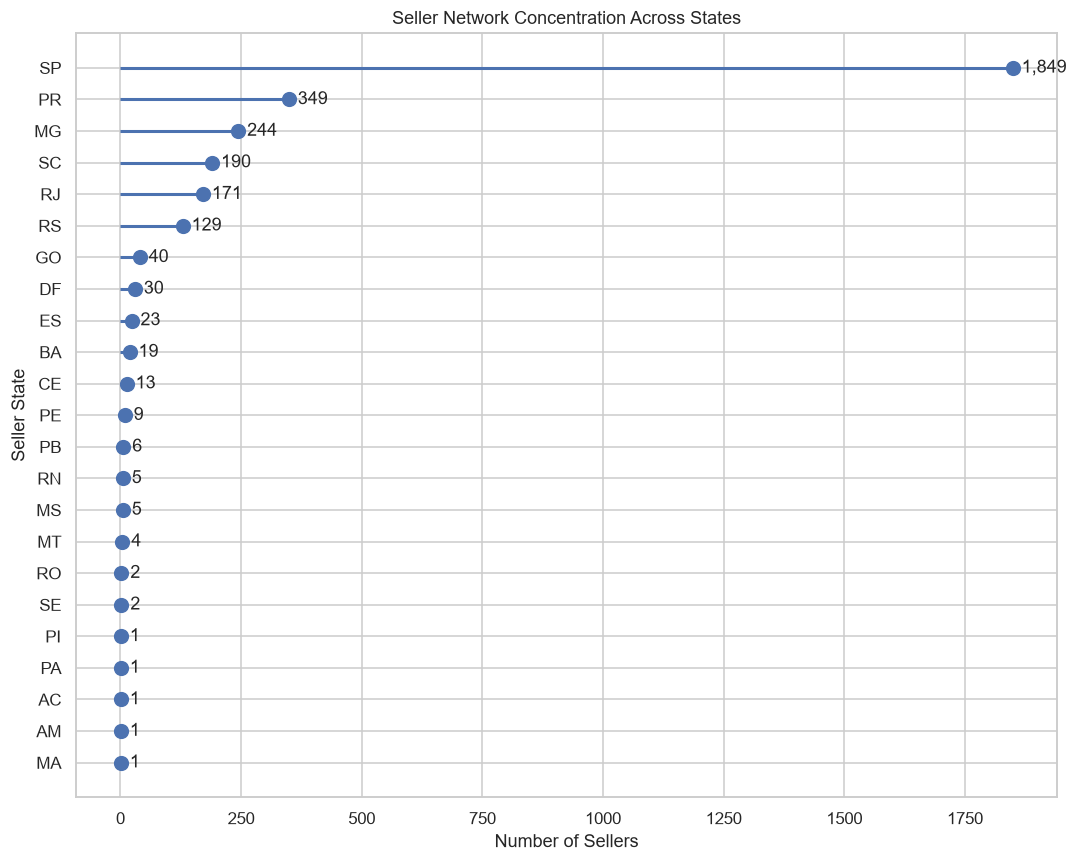
\includegraphics[width=0.7\textwidth]{figures/f_sellers_by_state_original.png}
    \caption{Sellers by state (original analysis).}
    \label{fig:sellers_orig}
\end{figure}

\begin{figure}[htbp]
    \centering
    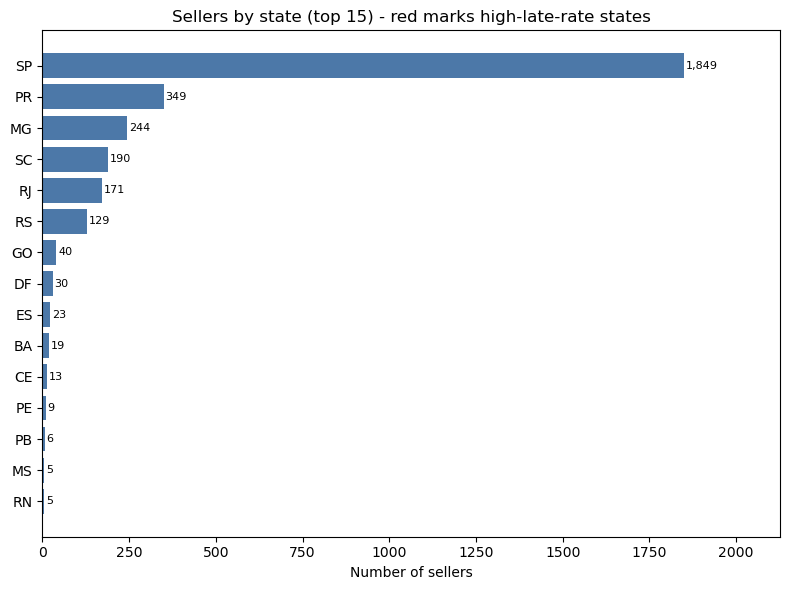
\includegraphics[width=0.75\textwidth]{figures/f_sellers_by_state_recompute.png}
    \caption{Sellers by state, top 15 (live recomputation). States highlighted in red are the
    same high-late-rate states from Figure~\ref{fig:late_rate_recompute}.}
    \label{fig:sellers_recompute}
\end{figure}

Sellers are heavily concentrated in SP (1{,}849, 60\% of all sellers), far exceeding PR (349),
MG (244), SC (190), and RJ (171). Matching seller density against late-delivery rate confirms the
seller-density theory for the low-seller states -- \textbf{MA and PI have just 1 seller each}
locally -- but it does \emph{not} fully explain RJ: RJ has a substantial seller base (171 sellers,
third-most in the country) and still runs an 11.9\% late-delivery rate.

\takeaway{``Grow the local seller base'' is a well-supported lever for AL, MA, PI, and CE. RJ's
problem is more likely logistics- or carrier-side and needs separate investigation (e.g.\ carrier
mix, warehouse location) rather than the same seller-recruitment fix applied everywhere.}

\section{Seller-Level Quality Issues}

Joining raw order items, products, and review-topic mining, sellers with more than 100 deliveries
were ranked by the share of their orders flagged with a ``product quality'' complaint
(Figures~\ref{fig:quality_sellers_orig}--\ref{fig:quality_sellers_recompute}).

\begin{figure}[htbp]
    \centering
    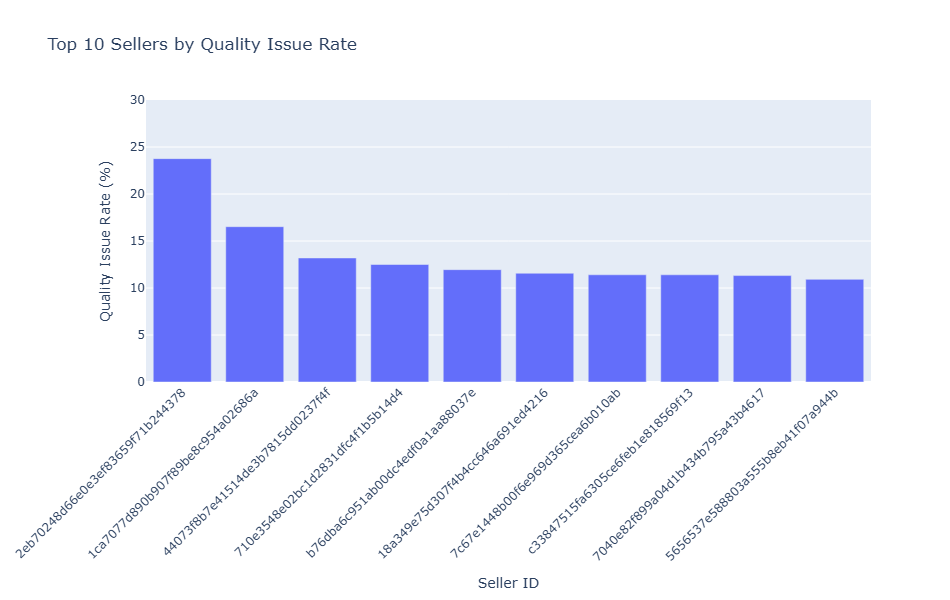
\includegraphics[width=0.7\textwidth]{figures/f_top10_quality_sellers_original.png}
    \caption{Top 10 sellers by quality-issue rate (original interactive analysis).}
    \label{fig:quality_sellers_orig}
\end{figure}

\begin{figure}[htbp]
    \centering
    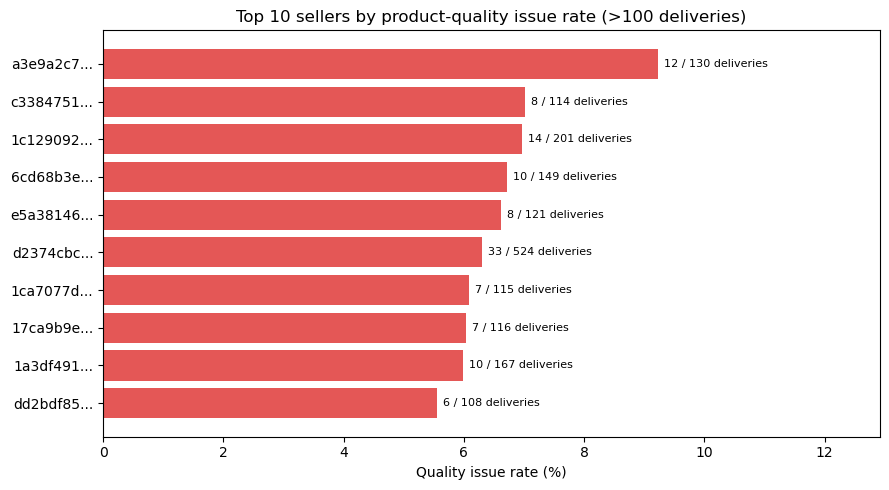
\includegraphics[width=0.75\textwidth]{figures/f_top10_quality_sellers_recompute.png}
    \caption{Top 10 sellers by quality-issue rate, live recomputation against current review-mining
    output.}
    \label{fig:quality_sellers_recompute}
\end{figure}

The current live-recomputed top seller has a \textbf{9.23\%} quality-issue rate (12 issues out of
130 deliveries); several others sit above 5\%.

\caveat{An earlier draft of this analysis cited a top rate of 23.76\% (48 of 202 deliveries) based
on a stale run of the review-mining pipeline. Re-running the identical join logic against the
current \path{processed_customer_reviews.csv} produced the 9.23\% figure reported here. This
table is intentionally kept as a live, re-runnable computation (rather than a static exported
chart) specifically so it cannot silently drift out of date again.}

\takeaway{This is a small, identifiable group of sellers. A targeted quality audit or
corrective-action program aimed at this handful of sellers would disproportionately reduce
product-quality complaints without requiring a marketplace-wide policy change.}

\section{Product Category Analysis}

Restricting to categories with at least 500 orders (Figure~\ref{fig:quality_categories}),
\textbf{bed_bath_table} has the highest quality-issue rate at \textbf{5.2\%}, followed by
\textbf{luggage_accessories} (4.8\%) and \textbf{office_furniture} (4.5\%);
\textbf{furniture_decor}, \textbf{housewares}, and \textbf{telephony} also sit above 3\%.

\begin{figure}[htbp]
    \centering
    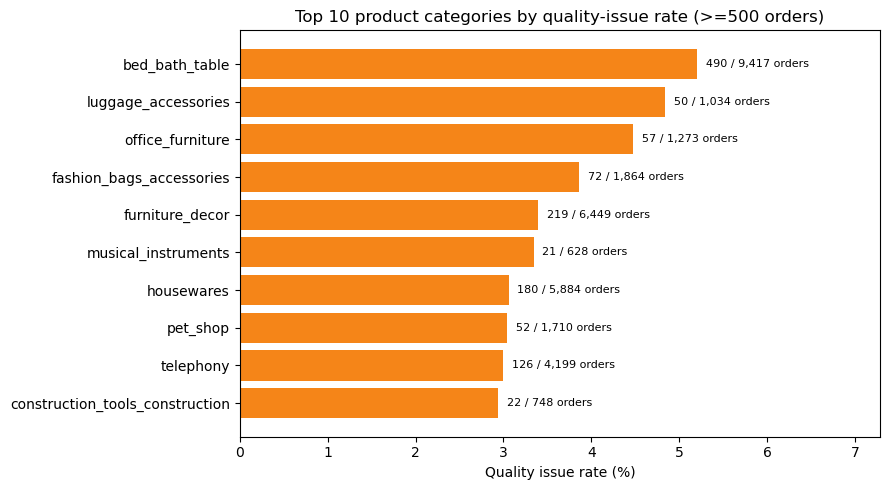
\includegraphics[width=0.75\textwidth]{figures/f_top10_quality_categories.png}
    \caption{Top 10 product categories by quality-issue rate ($\geq$500 orders).}
    \label{fig:quality_categories}
\end{figure}

\finding{The highest-risk categories are, notably, mostly bulky or fragile physical goods
(furniture, bags/luggage, home goods) -- the kind of product where damage-in-transit or a mismatch
between photos and the real item is more likely than for something like electronics accessories.}

\takeaway{This gives the platform a concrete, product-level lever alongside the seller-level one:
category-specific quality guidelines (packaging standards for bulky/fragile items, clearer
size/material listings) could reduce complaints in exactly the categories most prone to them,
rather than a single blanket policy applied to every seller regardless of what they sell.}

\section{Where Do Sellers Come From? The Acquisition Funnel}

\begin{figure}[htbp]
    \centering
    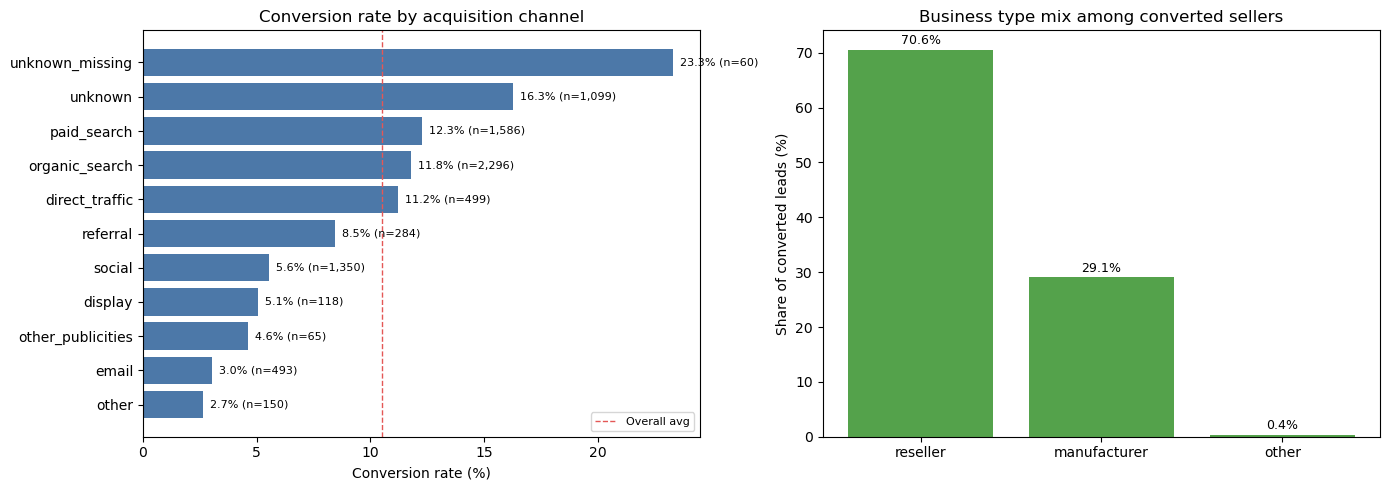
\includegraphics[width=0.9\textwidth]{figures/f_acquisition_funnel.png}
    \caption{Conversion rate by acquisition channel (left) and business-type mix among converted
    sellers (right).}
    \label{fig:funnel}
\end{figure}

Only about \textbf{10.5\%} of marketing-qualified leads ever convert into an active seller.
\path{organic_search} and \path{paid_search} bring in the most leads by volume, but they are
not the channels that convert best -- \path{paid_search} and untracked/\path{unknown} referral
sources actually convert at a higher rate, while high-volume channels like \path{social} and
\path{email} convert well below average. Among sellers who do convert, \textbf{resellers
outnumber manufacturers roughly 2:1}.

\takeaway{If the platform wants better sellers (not just more of them), the acquisition budget is
currently weighted toward channels that bring in volume, not necessarily the channels that convert
best or attract the kind of seller least likely to end up in the quality-issue or high-late-rate
groups identified above. Confirming that link directly (joining converted \path{seller_id}s back
to seller performance) is a natural next step not yet completed here.}

\section{Closing the Loop: Sizing the Priority Segment}

The analysis started with one question: why do only 3.1\% of customers ever come back? Every
section since has chased a piece of the answer. The final step sizes the customers this actually
affects, so the recommendation is concrete rather than abstract.

\begin{figure}[htbp]
    \centering
    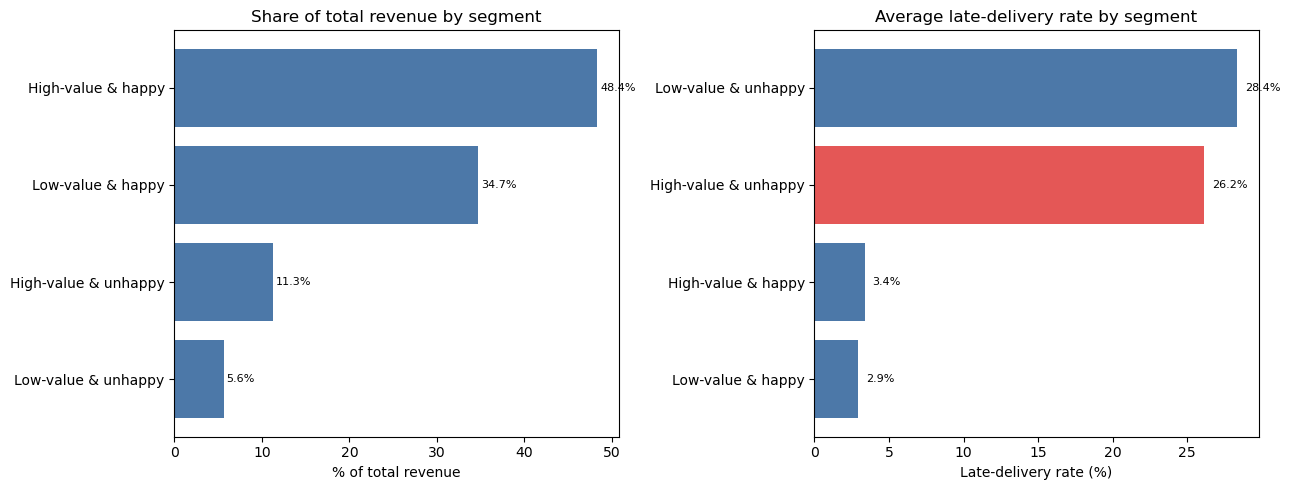
\includegraphics[width=0.9\textwidth]{figures/f_customer_quadrants.png}
    \caption{Customer base split into four value $\times$ satisfaction quadrants: revenue share
    (left) and average late-delivery rate (right) by segment.}
    \label{fig:quadrants}
\end{figure}

Splitting all customers by value (top-quartile spend vs.\ not) and satisfaction (average review
score $\leq 2$ vs.\ not) produces four segments:

\begin{center}
\begin{tabular}{lrrr}
\toprule
\textbf{Segment} & \textbf{Customers} & \textbf{Revenue Share} & \textbf{Late-Delivery Rate} \\
\midrule
High-value \& happy   & 19{,}835 & 48.4\% & 3\%  \\
Low-value \& happy    & 62{,}384 & 34.7\% & 3\%  \\
High-value \& unhappy & 4{,}194  & 11.3\% & 26\% \\
Low-value \& unhappy  & 9{,}683  & 5.6\%  & 28\% \\
\bottomrule
\end{tabular}
\end{center}

\finding{The two ``happy'' segments together hold 83\% of all revenue at a \textasciitilde3\%
late-rate -- this is the healthy core of the business and the benchmark to protect. The two
``unhappy'' segments run late-delivery rates roughly 8--9x higher than their happy counterparts.
This is the whole thesis of the analysis in one table: dissatisfaction is not evenly spread across
the customer base, it is concentrated in a delivery-driven minority.}

\takeaway{The \textbf{high-value \& unhappy} segment (\textasciitilde4{,}200 customers, 11.3\% of
revenue, \textasciitilde26\% late-delivery rate vs.\ \textasciitilde3\% for high-value \& happy
customers) is the single highest-leverage place to intervene first: fixing their delivery
experience protects real revenue without requiring a platform-wide overhaul.}

\section{Delivery Delay and Repeat Behavior}

\begin{figure}[htbp]
    \centering
    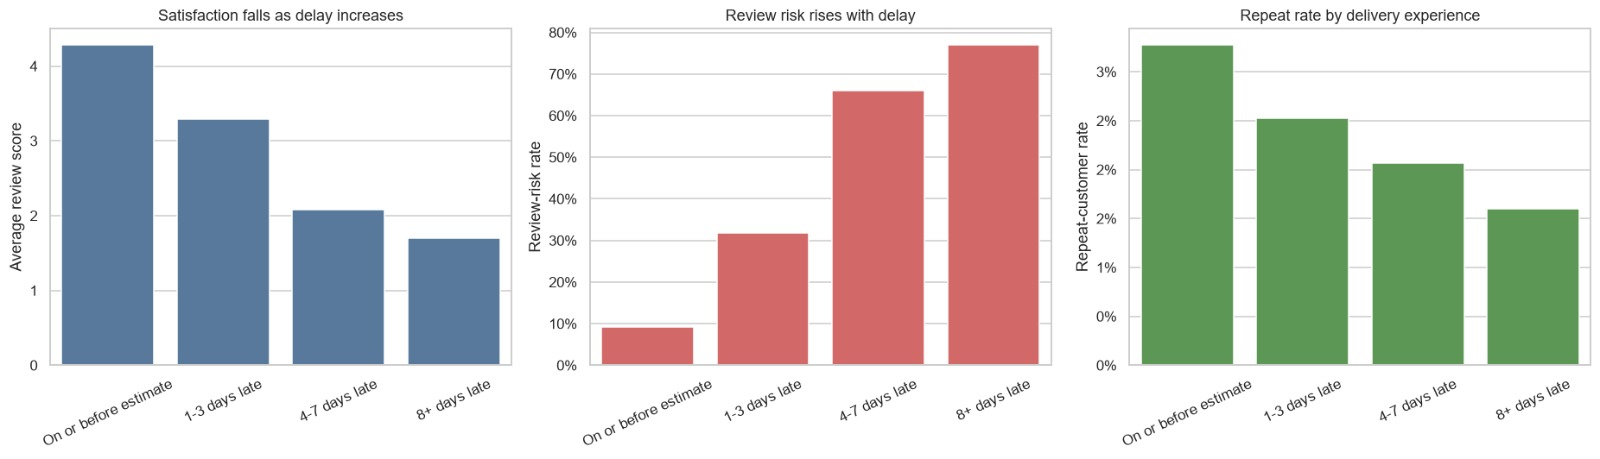
\includegraphics[width=0.85\textwidth]{figures/f_delay_repeat_original.jpeg}
    \caption{Customer satisfaction vs.\ delivery delay (original analysis).}
    \label{fig:delay_orig}
\end{figure}

\begin{figure}[htbp]
    \centering
    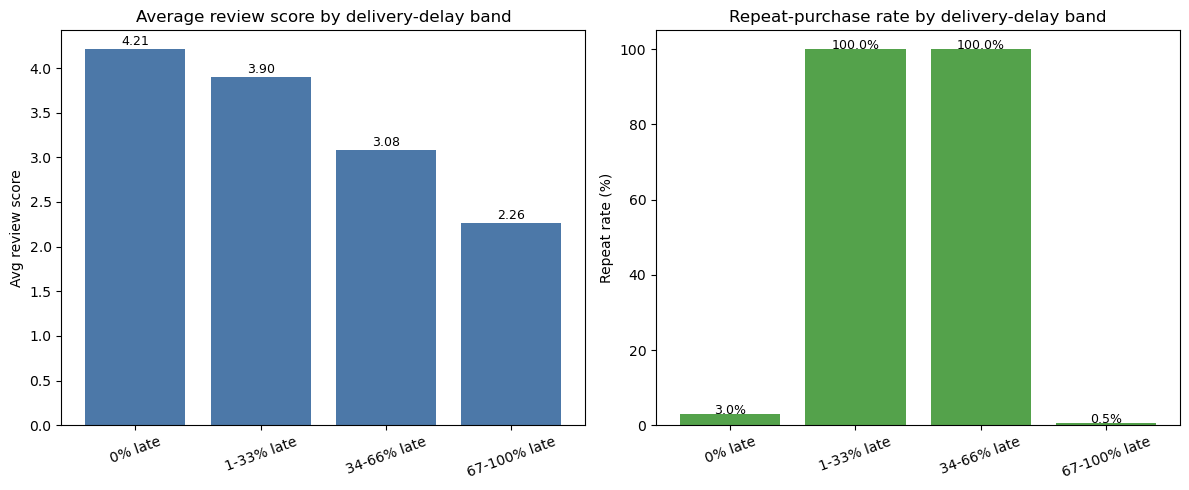
\includegraphics[width=0.85\textwidth]{figures/f_delay_band_recompute.png}
    \caption{Average review score (left) and repeat-purchase rate (right) by delivery-delay band,
    live recomputation.}
    \label{fig:delay_recompute}
\end{figure}

Bucketing customers by their average late-delivery rate confirms the intended pattern cleanly on
the two largest bands: customers who never experienced a late delivery (89{,}597 customers) repeat
at \textbf{3.0\%}, while customers whose only/all deliveries were late (6{,}214 customers) repeat
at just \textbf{0.5\%} -- a real, large gap.

\caveat{The two middle bands (``1--33\% late'', ``34--66\% late'') show a 100\% repeat rate in the
raw output, but this is a \textbf{sample-composition artifact, not a genuine finding}: a customer
can only have a \emph{fractional} late-delivery rate at all (e.g.\ 33\% = 1 late order out of 3) if
they placed 2+ orders in the first place -- so by construction, only repeat customers can ever land
in these two middle bands, and they are also tiny (26 and 259 customers respectively, versus tens
of thousands in the other two bands). These two bars are excluded from the causal story and shown
only for transparency about the full distribution. This is a methodological trap worth calling out
explicitly in any presentation of this chart, since a naive reading would suggest delay
\emph{increases} repeat purchasing, which is the opposite of the well-supported conclusion.}

\clearpage

% ================================================================
\chapter{Recommendations}
% ================================================================

Based on the evidence assembled in Chapter 4, five recommendations are proposed, ordered by
expected leverage:

\begin{enumerate}[leftmargin=2em]
    \item \textbf{Delivery-promise SLA, protecting the high-value-unhappy cohort first.} The
        clearest, most consistent driver of dissatisfaction across every cut of the data (order,
        customer, seller, state) is delivery delay -- fix this first and other levers follow.
    \item \textbf{Targeted seller and category quality program}, not a blanket policy -- audit the
        small group of consistently high-issue-rate sellers identified in Section~4.5, and set
        category-specific packaging/description standards for bulky or fragile goods
        (bed_bath_table, luggage, furniture, home goods) identified in Section~4.6.
    \item \textbf{Regional logistics intervention in high-late-rate, low-seller-density states}
        (AL, MA, PI), while treating SP as the operational benchmark to protect, not fix. RJ
        requires a separate, logistics/carrier-focused investigation given its adequate seller
        density.
    \item \textbf{Second-order retention nudge conditioned on a clean first delivery} -- the data
        shows delivery experience is where the platform is most likely to lose a customer for
        good.
    \item \textbf{Revisit acquisition channel mix} -- channels such as \path{social} and
        \path{email} carry real lead volume but convert well below the funnel average;
        reallocating spend toward better-converting channels could improve seller quality at the
        source, not just after the fact.
\end{enumerate}

\section*{A Note on Causality}
Every finding in this report is an \textit{association}, not a proven cause. Delivery delay
correlates strongly and consistently with dissatisfaction across every level of the data examined
-- order, customer, seller, and (more weakly) category -- which is the strongest kind of evidence a
purely observational analysis of this kind can offer. However, a seller or customer with other,
unrelated problems could plausibly show both symptoms (delay and dissatisfaction) independently of
one another, without one causing the other. The recommendations above should be read as the
most well-supported next actions to \emph{test} operationally (e.g.\ via a controlled delivery-SLA
pilot), not as settled facts to act on blindly.

\clearpage

% ================================================================
\chapter{Limitations}
% ================================================================

\begin{itemize}[leftmargin=2em]
    \item \textbf{Observational, not experimental data.} No finding in this report should be read
        as a controlled causal estimate; see the Note on Causality above.
    \item \textbf{Fixed observation window.} The customer-level repeat-purchase rate
        (\textasciitilde3.1\%) is a lower bound partly shaped by the dataset's fixed time window --
        customers who joined near the end of the observed period have had less opportunity to
        place a second order.
    \item \textbf{Small-sample segments.} Several cuts used in this report (3+-seller orders, 59
        orders; sellers with $>$100 deliveries in the quality-issue analysis; the two middle
        delivery-delay bands in Section~4.7) are small in absolute terms and should be treated as
        directionally useful, not statistically precise.
    \item \textbf{Marketing-funnel revenue fields are largely unusable.} 95\% of converted deals in
        the marketing-funnel table have a placeholder (originally 0, recoded to \path{NaN})
        declared-revenue value; only 5.3\% carry a genuine figure, so revenue-based funnel
        segmentation is illustrative at best.
    \item \textbf{Category-level dilution.} Aggregating to the category level weakens the
        delivery--satisfaction correlation considerably compared to the order or seller level, so
        category-level correlations should not be used in isolation to rule delivery in or out as a
        cause within a specific category.
    \item \textbf{Known data-quality flag.} \path{active_seller_flag} in the seller-level table
        is uniformly \path{True} and should not be used for active/inactive filtering until fixed
        upstream.
\end{itemize}

\clearpage

% ================================================================
\chapter{Conclusion}
% ================================================================

This project traced a single, well-supported causal hypothesis -- \emph{delivery unreliability
drives dissatisfaction, and dissatisfaction drives non-return} -- through every table in the
dataset, from raw cleaning decisions through order-, customer-, seller-, and category-level
exploratory analysis, to a specific, revenue-sized recommendation. The evidence is unusually
consistent across levels of analysis: the same delivery-delay signal appears, at similar
magnitude, whether measured at the order, customer, or seller grain. At the same time, the
analysis surfaced genuine nuance that a single top-line number would have missed -- RJ's reliability
problem hiding inside a large market, the sample-composition artifact in the delay-band repeat-rate
chart, and the category-level dilution of the delivery signal -- each of which changes what the
\emph{right} intervention looks like. The recommendations in Chapter 5 are offered as the
best-supported next actions for the marketplace to test, with the explicit caveat that this is an
observational study and the next step for any of these levers is a controlled pilot, not a
platform-wide rollout.

\clearpage

% ================================================================
\appendix
\chapter{Appendix: Codebase, Artifacts, and Supporting Documents}
% ================================================================

\section{Code Repository}
The complete codebase, including every notebook and script referenced in this report, is version
controlled and publicly available on GitHub:

\begin{center}
\url{https://github.com/Hiteshpanghal900/ecommerce-visual-analytics}
\end{center}

\noindent The repository includes:
\begin{itemize}[leftmargin=2em]
    \item All data-cleaning notebooks (\path{data_cleaning/})
    \item All exploratory-analysis notebooks (\path{EDA/}, \path{data-visualization/})
    \item The combined explanatory narrative notebook, \path{combined_eda.ipynb}, from which
        this report's Chapter~4 is drawn
    \item An interactive Plotly Dash dashboard (\path{dashboard/app.py}) for exploring the
        cleaned tables visually
    \item The per-table question-and-answer reference documents (\path{questions_ans_by_table/})
    \item \path{requirements.txt} for reproducing the Python environment
\end{itemize}

\section{Key Files Referenced in This Report}
\begin{itemize}[leftmargin=2em]
    \item \textbf{Narrative source:} \path{combined_eda.ipynb}
    \item \textbf{Cleaning notebooks:}
        \path{data_cleaning/cleaning_master_order_table.ipynb},
        \path{data_cleaning/clean_seller_master_table.ipynb},
        \path{data_cleaning/clean_category_master_table.ipynb},
        \path{data_cleaning/clean_marketing_funnel_table.ipynb}
    \item \textbf{EDA notebooks:}
        \path{EDA/eda_orders.ipynb}, \path{EDA/eda_master_orders_table.ipynb},
        \path{EDA/eda_seller_master_table.ipynb},
        \path{EDA/marketing-funnel-analysis.ipynb},
        \path{EDA/review_message_analysis.ipynb},
        \path{data-visualization/customer-master-analysis.ipynb},
        \path{data-visualization/seller_product_analysis.ipynb}
    \item \textbf{Per-table Q\&A reference documents:}
        \path{questions_ans_by_table/orders_table1.md},
        \path{questions_ans_by_table/orders_table2_questions.md},
        \path{questions_ans_by_table/seller_table_questions.md},
        \path{questions_ans_by_table/customer_table_questions.md},
        \path{questions_ans_by_table/category_table_questions.md},
        \path{questions_ans_by_table/marketing_funnel_table_questions.md}
    \item \textbf{Interactive dashboard:} \path{dashboard/app.py} (see
        \path{dashboard/README.md} for run instructions)
\end{itemize}

\section{Reproducing This Report}
The figures embedded in this report were extracted directly from the executed outputs of
\path{combined_eda.ipynb}. To reproduce them: clone the repository above, install dependencies
from \path{requirements.txt}, and execute \path{combined_eda.ipynb} end to end (e.g.\ via
\path{jupyter nbconvert --to notebook --execute --inplace combined_eda.ipynb}); all figures and
printed numbers in this report will regenerate identically from the current data.

\end{document}
